% Options for packages loaded elsewhere
\PassOptionsToPackage{unicode}{hyperref}
\PassOptionsToPackage{hyphens}{url}
%
\documentclass[
]{article}
\usepackage{amsmath,amssymb}
\usepackage{lmodern}
\usepackage{iftex}
\ifPDFTeX
  \usepackage[T1]{fontenc}
  \usepackage[utf8]{inputenc}
  \usepackage{textcomp} % provide euro and other symbols
\else % if luatex or xetex
  \usepackage{unicode-math}
  \defaultfontfeatures{Scale=MatchLowercase}
  \defaultfontfeatures[\rmfamily]{Ligatures=TeX,Scale=1}
\fi
% Use upquote if available, for straight quotes in verbatim environments
\IfFileExists{upquote.sty}{\usepackage{upquote}}{}
\IfFileExists{microtype.sty}{% use microtype if available
  \usepackage[]{microtype}
  \UseMicrotypeSet[protrusion]{basicmath} % disable protrusion for tt fonts
}{}
\makeatletter
\@ifundefined{KOMAClassName}{% if non-KOMA class
  \IfFileExists{parskip.sty}{%
    \usepackage{parskip}
  }{% else
    \setlength{\parindent}{0pt}
    \setlength{\parskip}{6pt plus 2pt minus 1pt}}
}{% if KOMA class
  \KOMAoptions{parskip=half}}
\makeatother
\usepackage{xcolor}
\usepackage[margin=1in]{geometry}
\usepackage{color}
\usepackage{fancyvrb}
\newcommand{\VerbBar}{|}
\newcommand{\VERB}{\Verb[commandchars=\\\{\}]}
\DefineVerbatimEnvironment{Highlighting}{Verbatim}{commandchars=\\\{\}}
% Add ',fontsize=\small' for more characters per line
\usepackage{framed}
\definecolor{shadecolor}{RGB}{248,248,248}
\newenvironment{Shaded}{\begin{snugshade}}{\end{snugshade}}
\newcommand{\AlertTok}[1]{\textcolor[rgb]{0.94,0.16,0.16}{#1}}
\newcommand{\AnnotationTok}[1]{\textcolor[rgb]{0.56,0.35,0.01}{\textbf{\textit{#1}}}}
\newcommand{\AttributeTok}[1]{\textcolor[rgb]{0.77,0.63,0.00}{#1}}
\newcommand{\BaseNTok}[1]{\textcolor[rgb]{0.00,0.00,0.81}{#1}}
\newcommand{\BuiltInTok}[1]{#1}
\newcommand{\CharTok}[1]{\textcolor[rgb]{0.31,0.60,0.02}{#1}}
\newcommand{\CommentTok}[1]{\textcolor[rgb]{0.56,0.35,0.01}{\textit{#1}}}
\newcommand{\CommentVarTok}[1]{\textcolor[rgb]{0.56,0.35,0.01}{\textbf{\textit{#1}}}}
\newcommand{\ConstantTok}[1]{\textcolor[rgb]{0.00,0.00,0.00}{#1}}
\newcommand{\ControlFlowTok}[1]{\textcolor[rgb]{0.13,0.29,0.53}{\textbf{#1}}}
\newcommand{\DataTypeTok}[1]{\textcolor[rgb]{0.13,0.29,0.53}{#1}}
\newcommand{\DecValTok}[1]{\textcolor[rgb]{0.00,0.00,0.81}{#1}}
\newcommand{\DocumentationTok}[1]{\textcolor[rgb]{0.56,0.35,0.01}{\textbf{\textit{#1}}}}
\newcommand{\ErrorTok}[1]{\textcolor[rgb]{0.64,0.00,0.00}{\textbf{#1}}}
\newcommand{\ExtensionTok}[1]{#1}
\newcommand{\FloatTok}[1]{\textcolor[rgb]{0.00,0.00,0.81}{#1}}
\newcommand{\FunctionTok}[1]{\textcolor[rgb]{0.00,0.00,0.00}{#1}}
\newcommand{\ImportTok}[1]{#1}
\newcommand{\InformationTok}[1]{\textcolor[rgb]{0.56,0.35,0.01}{\textbf{\textit{#1}}}}
\newcommand{\KeywordTok}[1]{\textcolor[rgb]{0.13,0.29,0.53}{\textbf{#1}}}
\newcommand{\NormalTok}[1]{#1}
\newcommand{\OperatorTok}[1]{\textcolor[rgb]{0.81,0.36,0.00}{\textbf{#1}}}
\newcommand{\OtherTok}[1]{\textcolor[rgb]{0.56,0.35,0.01}{#1}}
\newcommand{\PreprocessorTok}[1]{\textcolor[rgb]{0.56,0.35,0.01}{\textit{#1}}}
\newcommand{\RegionMarkerTok}[1]{#1}
\newcommand{\SpecialCharTok}[1]{\textcolor[rgb]{0.00,0.00,0.00}{#1}}
\newcommand{\SpecialStringTok}[1]{\textcolor[rgb]{0.31,0.60,0.02}{#1}}
\newcommand{\StringTok}[1]{\textcolor[rgb]{0.31,0.60,0.02}{#1}}
\newcommand{\VariableTok}[1]{\textcolor[rgb]{0.00,0.00,0.00}{#1}}
\newcommand{\VerbatimStringTok}[1]{\textcolor[rgb]{0.31,0.60,0.02}{#1}}
\newcommand{\WarningTok}[1]{\textcolor[rgb]{0.56,0.35,0.01}{\textbf{\textit{#1}}}}
\usepackage{graphicx}
\makeatletter
\def\maxwidth{\ifdim\Gin@nat@width>\linewidth\linewidth\else\Gin@nat@width\fi}
\def\maxheight{\ifdim\Gin@nat@height>\textheight\textheight\else\Gin@nat@height\fi}
\makeatother
% Scale images if necessary, so that they will not overflow the page
% margins by default, and it is still possible to overwrite the defaults
% using explicit options in \includegraphics[width, height, ...]{}
\setkeys{Gin}{width=\maxwidth,height=\maxheight,keepaspectratio}
% Set default figure placement to htbp
\makeatletter
\def\fps@figure{htbp}
\makeatother
\setlength{\emergencystretch}{3em} % prevent overfull lines
\providecommand{\tightlist}{%
  \setlength{\itemsep}{0pt}\setlength{\parskip}{0pt}}
\setcounter{secnumdepth}{-\maxdimen} % remove section numbering
\ifLuaTeX
  \usepackage{selnolig}  % disable illegal ligatures
\fi
\IfFileExists{bookmark.sty}{\usepackage{bookmark}}{\usepackage{hyperref}}
\IfFileExists{xurl.sty}{\usepackage{xurl}}{} % add URL line breaks if available
\urlstyle{same} % disable monospaced font for URLs
\hypersetup{
  pdftitle={HUDM6026 Homework\_01},
  pdfauthor={Chenguang Pan},
  hidelinks,
  pdfcreator={LaTeX via pandoc}}

\title{HUDM6026 Homework\_01}
\author{Chenguang Pan}
\date{Jan 23, 2023}

\begin{document}
\maketitle

\hypertarget{question-01}{%
\subsection{Question 01}\label{question-01}}

\emph{A random variable X has a chi-square distribution with k degrees
of freedom (df) if it can be expressed as the sum of k independent
squared random normal variables. In that case, we write that
X\textasciitilde x2k. Write a function that has two arguments, n for
sample size and k for degrees of freedom. The purpose of the function is
to generate a random sample of size n from a x2k distribution.
Importantly, you may not use the rchisq suite of functions. Instead, use
\texttt{rnorm()} and the definition given above. }

\textbf{MY SOLUTION:}\\
Based on the chi-square distribution's definition, we randomly draw n
variables from a standard normal distribution for k times, and adds the
square sum of them, then the distribution of this sum will follow a
chi-square distribution. Based on this logic, I write a function
containing a for k-loop to simulate this process.

\begin{Shaded}
\begin{Highlighting}[]
\SpecialCharTok{\textgreater{}}\NormalTok{ my\_chisqr }\OtherTok{\textless{}{-}} \ControlFlowTok{function}\NormalTok{(n, k)\{}
\SpecialCharTok{+}   \CommentTok{\# create a vector with n 0s}
\SpecialCharTok{+}\NormalTok{   Q }\OtherTok{\textless{}{-}} \FunctionTok{rep}\NormalTok{(}\DecValTok{0}\NormalTok{,n)}
\SpecialCharTok{+}   \CommentTok{\# use a loop to k times sampling}
\SpecialCharTok{+}   \ControlFlowTok{for}\NormalTok{ (df }\ControlFlowTok{in} \FunctionTok{c}\NormalTok{(}\DecValTok{1}\SpecialCharTok{:}\NormalTok{k))\{}
\SpecialCharTok{+}     \CommentTok{\# create a vector of RVs from a standard normal distribution}
\SpecialCharTok{+}\NormalTok{     rv\_vec }\OtherTok{\textless{}{-}} \FunctionTok{rnorm}\NormalTok{(n, }\AttributeTok{mean =} \DecValTok{0}\NormalTok{, }\AttributeTok{sd =} \DecValTok{1}\NormalTok{)}
\SpecialCharTok{+}     \CommentTok{\# square the randomly RVs and adds them up within the for loop}
\SpecialCharTok{+}\NormalTok{     Q }\OtherTok{\textless{}{-}}\NormalTok{ Q }\SpecialCharTok{+}\NormalTok{ rv\_vec}\SpecialCharTok{\^{}}\DecValTok{2}
\SpecialCharTok{+}\NormalTok{   \}}
\SpecialCharTok{+}   \FunctionTok{return}\NormalTok{(Q)}
\SpecialCharTok{+}\NormalTok{ \}}
\end{Highlighting}
\end{Shaded}

\hypertarget{question-02}{%
\subsection{Question 02}\label{question-02}}

\emph{Use your function from above to generate a very large sample
(e.g., n = 1e7) from x23. Display the distribution of the sample by
creating a histogram in base or ggplot2. Play with the number of breaks
until you settle on a number that looks good. Then, use rchisq() to
generate a large sample of the same size and also create a histogram. If
your function is working correctly, the distributions should be very
nearly identical.}

\textbf{MY SOLUTION:}\\
I will test the function with \texttt{n\ =\ 1e7} and \texttt{k\ =\ 3}.
To ensure replication, using the random \texttt{set.seed(1000)} and
compare it with built-in function \texttt{rchisq()}.

\begin{Shaded}
\begin{Highlighting}[]
\SpecialCharTok{\textgreater{}} \FunctionTok{set.seed}\NormalTok{(}\DecValTok{1000}\NormalTok{)}
\SpecialCharTok{\textgreater{}}\NormalTok{ n\_size }\OtherTok{\textless{}{-}} \FloatTok{1e7}
\SpecialCharTok{\textgreater{}}\NormalTok{ k\_df }\OtherTok{\textless{}{-}} \DecValTok{3}
\SpecialCharTok{\textgreater{}} \CommentTok{\# using the function above to get the chi{-}square with n size and k degree freedom}
\ErrorTok{\textgreater{}}\NormalTok{ my\_chi }\OtherTok{\textless{}{-}} \FunctionTok{my\_chisqr}\NormalTok{(n\_size, k\_df)}
\SpecialCharTok{\textgreater{}} \CommentTok{\# plot the the results by using ggplot and plot(density) to make the figure looking good}
\ErrorTok{\textgreater{}} \FunctionTok{par}\NormalTok{(}\AttributeTok{mfrow =} \FunctionTok{c}\NormalTok{(}\DecValTok{2}\NormalTok{,}\DecValTok{2}\NormalTok{))}
\SpecialCharTok{\textgreater{}} \CommentTok{\# draw the histogram}
\ErrorTok{\textgreater{}} \FunctionTok{hist}\NormalTok{(my\_chi, }\AttributeTok{breaks=}\DecValTok{20}\NormalTok{, }\AttributeTok{main =} \StringTok{"My Chi{-}square"}\NormalTok{)}
\SpecialCharTok{\textgreater{}} \FunctionTok{hist}\NormalTok{(}\FunctionTok{rchisq}\NormalTok{(n\_size, k\_df), }\AttributeTok{breaks =} \DecValTok{20}\NormalTok{, }\AttributeTok{main =} \StringTok{"R Built{-}in Chi{-}square"}\NormalTok{)}
\SpecialCharTok{\textgreater{}} \FunctionTok{plot}\NormalTok{(}\FunctionTok{density}\NormalTok{(my\_chi), }\AttributeTok{col =} \StringTok{"blue"}\NormalTok{,}
\SpecialCharTok{+}      \AttributeTok{main =} \StringTok{"My Chi{-}square "}\NormalTok{,}
\SpecialCharTok{+}      \AttributeTok{xlab =} \StringTok{\textquotesingle{}n=1e7, k=3\textquotesingle{}}\NormalTok{,}
\SpecialCharTok{+}      \AttributeTok{ylab =} \StringTok{\textquotesingle{}Density\textquotesingle{}}\NormalTok{)}
\SpecialCharTok{\textgreater{}} \FunctionTok{plot}\NormalTok{(}\FunctionTok{density}\NormalTok{(}\FunctionTok{rchisq}\NormalTok{(n\_size, k\_df)), }\AttributeTok{col =} \StringTok{"red"}\NormalTok{,}
\SpecialCharTok{+}      \AttributeTok{main =} \StringTok{"R Built{-}in Chi{-}square"}\NormalTok{,}
\SpecialCharTok{+}      \AttributeTok{xlab =} \StringTok{\textquotesingle{}n=1e7, k=3\textquotesingle{}}\NormalTok{,}
\SpecialCharTok{+}      \AttributeTok{ylab =} \StringTok{\textquotesingle{}Density\textquotesingle{}}\NormalTok{)}
\SpecialCharTok{\textgreater{}} \CommentTok{\# to add a main title for all four graphs}
\ErrorTok{\textgreater{}} \FunctionTok{mtext}\NormalTok{(}\StringTok{"Figure 1. Graphs For Question 2"}\NormalTok{,}
\SpecialCharTok{+}       \AttributeTok{side =} \DecValTok{3}\NormalTok{,}
\SpecialCharTok{+}       \AttributeTok{line =} \SpecialCharTok{{-}}\DecValTok{1}\NormalTok{,}
\SpecialCharTok{+}       \AttributeTok{outer =}\NormalTok{ T)}
\end{Highlighting}
\end{Shaded}

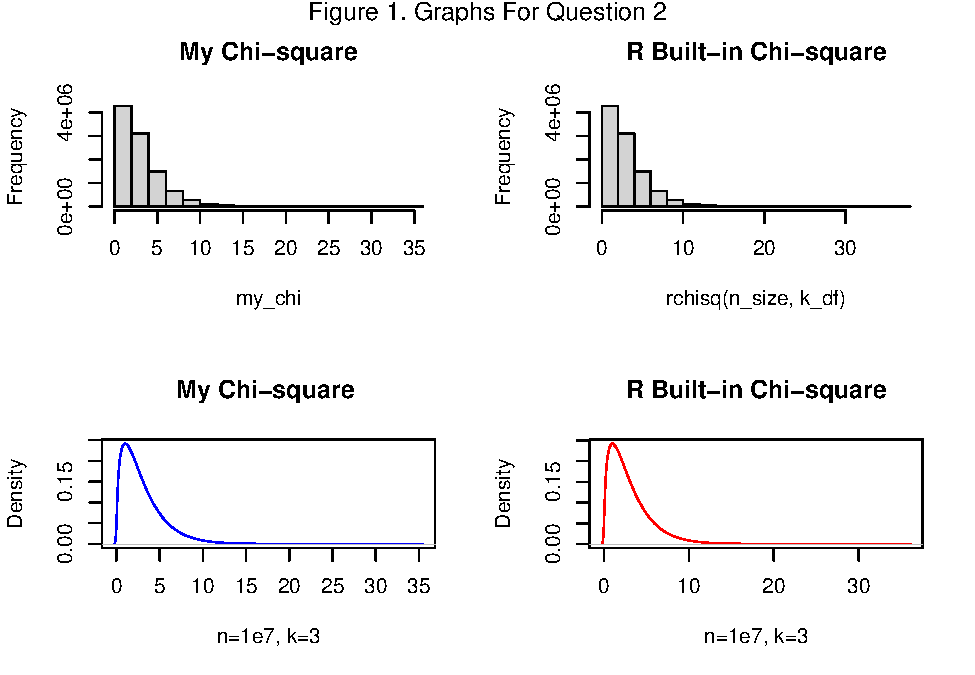
\includegraphics[width=1\linewidth,height=0.7\textheight]{homework_01_solutions_files/figure-latex/unnamed-chunk-2-1}
These figures shows that my function works well and the results are
identical to the R built-in function \texttt{rchisq()}.

\hypertarget{question-03}{%
\subsection{Question 03}\label{question-03}}

\emph{The chi-square distribution with 1 df is skewed heavily to the
right. Generate 10000 sample means from iid samples of x21 of size n = 5
and plot the distribution of the sample means using a histogram or other
univariate density plotting method. Then do the same for n = 10, n = 20,
and n = 40. Superimpose a normal curve with mean equal to sample mean of
the means and variance equal to sample variance of the means for each
plot. Discuss whether this progression demonstrates the LLNs or the CLT
and why.}

\textbf{MY SOLUTION:}

First, I will write a funciton to draw sample for 10000 times from a
chi-square distribution with the size of \texttt{size} and
\texttt{k\ =\ 1}. Then, calculate the sample means. That is, this
function will return the 10000 samples' means.

\begin{Shaded}
\begin{Highlighting}[]
\SpecialCharTok{\textgreater{}} \CommentTok{\# create a vector to load the 1e5 means}
\ErrorTok{\textgreater{}}\NormalTok{ means\_set }\OtherTok{\textless{}{-}} \FunctionTok{rep}\NormalTok{(}\DecValTok{0}\NormalTok{, }\DecValTok{10000}\NormalTok{)}
\SpecialCharTok{\textgreater{}} \CommentTok{\# use a for loop to draw sample for 1e5 times}
\ErrorTok{\textgreater{}}\NormalTok{ get\_means }\OtherTok{\textless{}{-}} \ControlFlowTok{function}\NormalTok{(size)\{ }
\SpecialCharTok{+}   \ControlFlowTok{for}\NormalTok{ (i }\ControlFlowTok{in} \FunctionTok{c}\NormalTok{(}\DecValTok{1}\SpecialCharTok{:}\DecValTok{10000}\NormalTok{)) \{}
\SpecialCharTok{+}     \CommentTok{\# draw a sample from a chisqr distribution with size and 1 df}
\SpecialCharTok{+}\NormalTok{     rv\_vec }\OtherTok{\textless{}{-}} \FunctionTok{rchisq}\NormalTok{(size, }\DecValTok{1}\NormalTok{)}
\SpecialCharTok{+}\NormalTok{     means\_set[i] }\OtherTok{\textless{}{-}} \FunctionTok{mean}\NormalTok{(rv\_vec)}
\SpecialCharTok{+}\NormalTok{   \}}
\SpecialCharTok{+}   \FunctionTok{return}\NormalTok{(means\_set)}
\SpecialCharTok{+}\NormalTok{ \} }
\end{Highlighting}
\end{Shaded}

This function \texttt{get\_means()}runs well. Then, I use a for-loop to
draw the four histograms.

From the following four histograms, one can see all the 10000 samples'
means converge at the peak. But the distribution of the means is not
followed a normal distribution. Therefore, these figures demonstrates
that LLNs rather than CLT.

\begin{Shaded}
\begin{Highlighting}[]
\SpecialCharTok{\textgreater{}} \FunctionTok{par}\NormalTok{(}\AttributeTok{mfrow =} \FunctionTok{c}\NormalTok{(}\DecValTok{2}\NormalTok{,}\DecValTok{2}\NormalTok{))}
\SpecialCharTok{\textgreater{}} \ControlFlowTok{for}\NormalTok{ (size\_ }\ControlFlowTok{in} \FunctionTok{c}\NormalTok{(}\DecValTok{5}\NormalTok{, }\DecValTok{10}\NormalTok{, }\DecValTok{20}\NormalTok{, }\DecValTok{40}\NormalTok{)) \{}
\SpecialCharTok{+}\NormalTok{   mean\_vec }\OtherTok{\textless{}{-}} \FunctionTok{get\_means}\NormalTok{(size\_)}
\SpecialCharTok{+}   \CommentTok{\# add argument prob = TRUE to draw density hist.}
\SpecialCharTok{+}   \FunctionTok{hist}\NormalTok{(mean\_vec, }\AttributeTok{prob =} \ConstantTok{TRUE}\NormalTok{, }\AttributeTok{breaks =} \DecValTok{10}\NormalTok{,}
\SpecialCharTok{+}        \AttributeTok{main =} \FunctionTok{paste}\NormalTok{(}\StringTok{"size="}\NormalTok{, }\FunctionTok{as.character}\NormalTok{(size\_)),}
\SpecialCharTok{+}        \AttributeTok{xlab =} \StringTok{"means"}\NormalTok{)}
\SpecialCharTok{+}\NormalTok{   x }\OtherTok{\textless{}{-}} \FunctionTok{seq}\NormalTok{(}\FunctionTok{min}\NormalTok{(mean\_vec),}\FunctionTok{max}\NormalTok{(mean\_vec), }\AttributeTok{length =} \FunctionTok{length}\NormalTok{(mean\_vec))}
\SpecialCharTok{+}\NormalTok{   f }\OtherTok{\textless{}{-}} \FunctionTok{dnorm}\NormalTok{(x, }\AttributeTok{mean =} \FunctionTok{mean}\NormalTok{(mean\_vec), }\AttributeTok{sd =} \FunctionTok{sd}\NormalTok{(mean\_vec))}
\SpecialCharTok{+}   \FunctionTok{lines}\NormalTok{(x,f, }\AttributeTok{col =} \StringTok{\textquotesingle{}red\textquotesingle{}}\NormalTok{, }\AttributeTok{lwd =} \DecValTok{1}\NormalTok{)}
\SpecialCharTok{+}\NormalTok{ \}}
\SpecialCharTok{\textgreater{}} \FunctionTok{mtext}\NormalTok{(}\StringTok{"Figure 2. Histograms For Question 3"}\NormalTok{,}
\SpecialCharTok{+}       \AttributeTok{side =} \DecValTok{3}\NormalTok{,}
\SpecialCharTok{+}       \AttributeTok{line =} \SpecialCharTok{{-}}\DecValTok{1}\NormalTok{,}
\SpecialCharTok{+}       \AttributeTok{outer =}\NormalTok{ T)}
\end{Highlighting}
\end{Shaded}

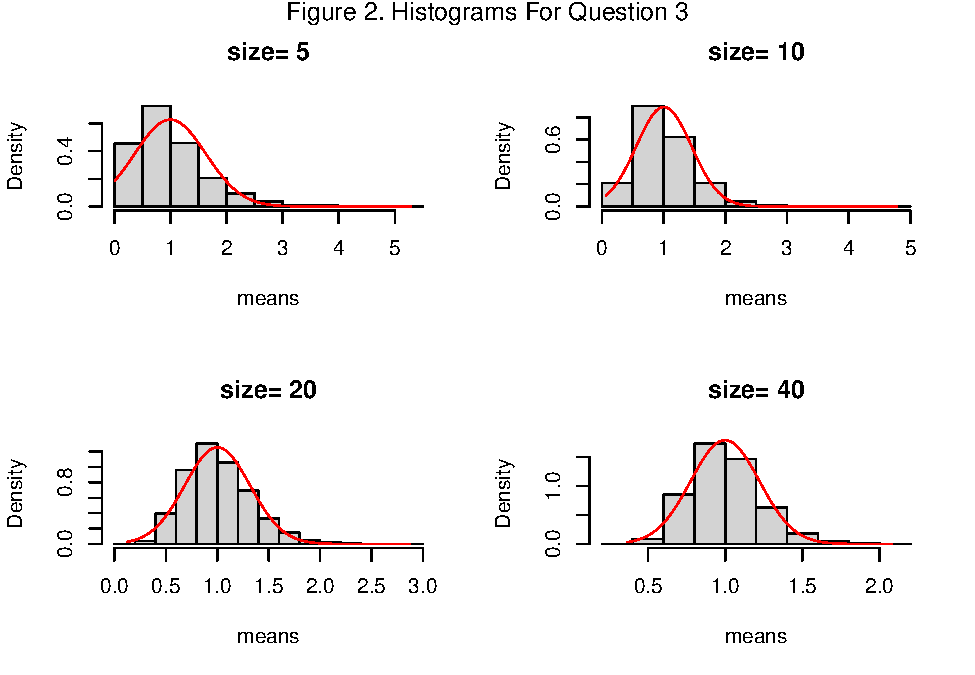
\includegraphics[width=1\linewidth,height=0.5\textheight]{homework_01_solutions_files/figure-latex/unnamed-chunk-4-1}

\hypertarget{question-04-bonous}{%
\subsection{Question 04 {[}bonous{]}}\label{question-04-bonous}}

\emph{Write a function to generate data (in a data frame or tibble) from
the following regression model.}

\textbf{MY SOLUTION:}\\
This question seems to be more challenging. I will write all my thoughts
behind my codes.

First things first, why we need to generate data based on the model's
assumption?
\href{https://towardsdatascience.com/generate-simulated-dataset-for-linear-model-in-r-469a5e2f4c2e}{This
website} mentioned: one of the main problems that the researchers
usually encountered when trying to implement the proposed model is the
lack of the proper real-world dataset that follows the model's
assumptions. Or in the other case, the real-world dataset exists, but
the dataset itself is very expensive and hard to collect.

The process of generating a simulated dataset can be explained as
follows. First, we specify the model that we want to simulate. Next, we
determine each independent variable's coefficient, then simulate the
independent variable and error that follows a probability distribution.
And finally, compute the dependent variable based on the simulated
independent variable (and its predetermined coefficient) and error.

Given that sovling this question need some knowledge about multivariate
normal distribution. I found it
\href{https://brilliant.org/wiki/multivariate-normal-distribution/?irclickid=zrX11zzxmxyNWr-WSkQQ6zQ1UkA1E6R2s2F1Uw0\&utm_medium=affiliates\&utm_campaign=1310690\&utm_source=\&utm_content=1674588816059_TEXT_LINK_20\%25\%20Off\%20Annual\%20Subscription\%20\&utm_term=middle\&irgwc=1}{here}
to refresh my understanding.

For the code, I made a function to generate data in matrix form.

\begin{Shaded}
\begin{Highlighting}[]
\SpecialCharTok{\textgreater{}} \CommentTok{\# import the package to run multivariate normal distribution}
\ErrorTok{\textgreater{}} 
\ErrorTok{\textgreater{}}\NormalTok{ data\_gen }\OtherTok{\textless{}{-}} \ControlFlowTok{function}\NormalTok{(n)\{}
\SpecialCharTok{+}   \FunctionTok{library}\NormalTok{(mvtnorm)}
\SpecialCharTok{+}   \CommentTok{\# define the covariance matrix of X1, X2, and X3}
\SpecialCharTok{+}   \CommentTok{\# note X1\textasciitilde{}X3 are all continuous variables.}
\SpecialCharTok{+}\NormalTok{   cov\_matrix }\OtherTok{\textless{}{-}} \FunctionTok{matrix}\NormalTok{(}\FunctionTok{c}\NormalTok{(}\FloatTok{13.6}\NormalTok{, }\SpecialCharTok{{-}}\FloatTok{14.5}\NormalTok{, }\SpecialCharTok{{-}}\FloatTok{103.4}\NormalTok{, }
\SpecialCharTok{+}                          \SpecialCharTok{{-}}\FloatTok{14.5}\NormalTok{, }\FloatTok{65.2}\NormalTok{, }\FloatTok{154.0}\NormalTok{,}
\SpecialCharTok{+}                          \SpecialCharTok{{-}}\FloatTok{103.4}\NormalTok{, }\FloatTok{154.0}\NormalTok{, }\FloatTok{2702.0}\NormalTok{),}\DecValTok{3}\NormalTok{,}\DecValTok{3}\NormalTok{)}
\SpecialCharTok{+}   \CommentTok{\# generate the X\textquotesingle{}s matrix using multivariate normal distribution}
\SpecialCharTok{+}\NormalTok{   X }\OtherTok{\textless{}{-}} \FunctionTok{rmvnorm}\NormalTok{(}\AttributeTok{n =}\NormalTok{ n, }\AttributeTok{sigma =}\NormalTok{ cov\_matrix) }\CommentTok{\# }\AlertTok{TODO}\CommentTok{: what about the means?}
\SpecialCharTok{+}   \CommentTok{\# X is a n * 3 matrix}
\SpecialCharTok{+}\NormalTok{   X1 }\OtherTok{\textless{}{-}}\NormalTok{ X[,}\DecValTok{1}\NormalTok{]; X2 }\OtherTok{\textless{}{-}}\NormalTok{ X[,}\DecValTok{2}\NormalTok{]; X3 }\OtherTok{\textless{}{-}}\NormalTok{ X[,}\DecValTok{3}\NormalTok{]}
\SpecialCharTok{+}   \CommentTok{\# generate the error term}
\SpecialCharTok{+}\NormalTok{   Error }\OtherTok{\textless{}{-}} \FunctionTok{rnorm}\NormalTok{(}\AttributeTok{n =}\NormalTok{ n, }\AttributeTok{mean =} \DecValTok{0}\NormalTok{, }\AttributeTok{sd =} \FloatTok{0.75}\NormalTok{)}
\SpecialCharTok{+}   \CommentTok{\# estimate the vector of dependent variable based on the model}
\SpecialCharTok{+}\NormalTok{   Y }\OtherTok{\textless{}{-}} \FloatTok{71.0} \SpecialCharTok{{-}} \FloatTok{0.28}\SpecialCharTok{*}\NormalTok{X1 }\SpecialCharTok{+} \FloatTok{0.05}\SpecialCharTok{*}\NormalTok{X2 }\SpecialCharTok{{-}} \FloatTok{0.007}\SpecialCharTok{*}\NormalTok{X3 }\SpecialCharTok{+}\NormalTok{ Error}
\SpecialCharTok{+}\NormalTok{   out }\OtherTok{\textless{}{-}} \FunctionTok{data.frame}\NormalTok{(X1,X2,X3,Y)}
\SpecialCharTok{+}   \FunctionTok{return}\NormalTok{(out)}
\SpecialCharTok{+}\NormalTok{ \}}
\end{Highlighting}
\end{Shaded}

This function runs well. Then, create a dataset with 1000 observations
and test the linear model.

\begin{Shaded}
\begin{Highlighting}[]
\SpecialCharTok{\textgreater{}} \FunctionTok{set.seed}\NormalTok{(}\DecValTok{666}\NormalTok{)}
\SpecialCharTok{\textgreater{}}\NormalTok{ data\_simulate }\OtherTok{\textless{}{-}} \FunctionTok{data\_gen}\NormalTok{(}\DecValTok{1000}\NormalTok{)}
\SpecialCharTok{\textgreater{}} \CommentTok{\# head(data\_simulate)}
\ErrorTok{\textgreater{}}\NormalTok{ lm\_est }\OtherTok{\textless{}{-}} \FunctionTok{lm}\NormalTok{(Y }\SpecialCharTok{\textasciitilde{}}\NormalTok{ X1 }\SpecialCharTok{+}\NormalTok{ X2 }\SpecialCharTok{+}\NormalTok{ X3, }\AttributeTok{data =}\NormalTok{ data\_simulate)}
\SpecialCharTok{\textgreater{}} \FunctionTok{summary}\NormalTok{(lm\_est)}

\NormalTok{Call}\SpecialCharTok{:}
\FunctionTok{lm}\NormalTok{(}\AttributeTok{formula =}\NormalTok{ Y }\SpecialCharTok{\textasciitilde{}}\NormalTok{ X1 }\SpecialCharTok{+}\NormalTok{ X2 }\SpecialCharTok{+}\NormalTok{ X3, }\AttributeTok{data =}\NormalTok{ data\_simulate)}

\NormalTok{Residuals}\SpecialCharTok{:}
\NormalTok{     Min       1Q   Median       3Q      Max }
\SpecialCharTok{{-}}\FloatTok{2.13684} \SpecialCharTok{{-}}\FloatTok{0.47060} \SpecialCharTok{{-}}\FloatTok{0.02534}  \FloatTok{0.50065}  \FloatTok{2.35442} 

\NormalTok{Coefficients}\SpecialCharTok{:}
\NormalTok{              Estimate Std. Error t value }\FunctionTok{Pr}\NormalTok{(}\SpecialCharTok{\textgreater{}}\ErrorTok{|}\NormalTok{t}\SpecialCharTok{|}\NormalTok{)    }
\NormalTok{(Intercept) }\FloatTok{70.9846997}  \FloatTok{0.0238692} \FloatTok{2973.90}   \SpecialCharTok{\textless{}}\FloatTok{2e{-}16} \SpecialCharTok{**}\ErrorTok{*}
\NormalTok{X1          }\SpecialCharTok{{-}}\FloatTok{0.2832359}  \FloatTok{0.0086811}  \SpecialCharTok{{-}}\FloatTok{32.63}   \SpecialCharTok{\textless{}}\FloatTok{2e{-}16} \SpecialCharTok{**}\ErrorTok{*}
\NormalTok{X2           }\FloatTok{0.0514251}  \FloatTok{0.0034581}   \FloatTok{14.87}   \SpecialCharTok{\textless{}}\FloatTok{2e{-}16} \SpecialCharTok{**}\ErrorTok{*}
\NormalTok{X3          }\SpecialCharTok{{-}}\FloatTok{0.0078670}  \FloatTok{0.0005578}  \SpecialCharTok{{-}}\FloatTok{14.11}   \SpecialCharTok{\textless{}}\FloatTok{2e{-}16} \SpecialCharTok{**}\ErrorTok{*}
\SpecialCharTok{{-}{-}{-}}
\NormalTok{Signif. codes}\SpecialCharTok{:}  \DecValTok{0} \StringTok{\textquotesingle{}***\textquotesingle{}} \FloatTok{0.001} \StringTok{\textquotesingle{}**\textquotesingle{}} \FloatTok{0.01} \StringTok{\textquotesingle{}*\textquotesingle{}} \FloatTok{0.05} \StringTok{\textquotesingle{}.\textquotesingle{}} \FloatTok{0.1} \StringTok{\textquotesingle{} \textquotesingle{}} \DecValTok{1}

\NormalTok{Residual standard error}\SpecialCharTok{:} \FloatTok{0.7541}\NormalTok{ on }\DecValTok{996}\NormalTok{ degrees of freedom}
\NormalTok{Multiple R}\SpecialCharTok{{-}}\NormalTok{squared}\SpecialCharTok{:}  \FloatTok{0.6807}\NormalTok{,    Adjusted R}\SpecialCharTok{{-}}\NormalTok{squared}\SpecialCharTok{:}  \FloatTok{0.6798} 
\NormalTok{F}\SpecialCharTok{{-}}\NormalTok{statistic}\SpecialCharTok{:} \FloatTok{707.8}\NormalTok{ on }\DecValTok{3}\NormalTok{ and }\DecValTok{996}\NormalTok{ DF,  p}\SpecialCharTok{{-}}\NormalTok{value}\SpecialCharTok{:} \ErrorTok{\textless{}} \FloatTok{2.2e{-}16}
\end{Highlighting}
\end{Shaded}

The results show that the estimated coefficient are \(\beta_0 = 70.98\),
\(\beta_1 = -0.28\),\(\beta_2 = 0.05\), \(\beta_3 = 0.008\), which are
pretty close to the coefficients the text given. The overall model can
significantly predict the outcome. All independent variables and
constant are statistically significant as well (based on the P-value at
the significant level of .05).

\end{document}
